\documentclass{article}
\usepackage[utf8]{inputenc}

\title{CSB: Coders Strike Back}
\author{Eivind Magnus Hvidevold}
\date{February 2019}

\usepackage{import}
\usepackage{natbib}
\usepackage{amsmath}
\usepackage{graphicx}
\usepackage{hyperref}
\hypersetup{
    colorlinks=true,
    linkcolor=blue,
    filecolor=magenta,      
    urlcolor=cyan,
}
\usepackage{tikz}
\usepackage{pgfplots}
\usepackage{xfp}
\usepackage{caption}
\usepackage{parskip}
\usepackage{subfiles}

\usepackage{listings}
\usepackage{xcolor}
\lstset { %
    language=C++,
    backgroundcolor=\color{black!5}, % set backgroundcolor
    basicstyle=\footnotesize,% basic font setting
}
\pgfplotsset{compat=1.15}

\usepackage{gensymb}

% \usepackage{expl3}
% \ExplSyntaxOn
% \cs_new_eq:NN \fpeval \fp_eval:n
% \ExplSyntaxOff
\protected\def\fpset#1#2{\edef#1{\fpeval{#2}}}

% \usepgfplotslibrary{external}

% \tikzexternalize

\setlength\parindent{0pt}

\usepackage{csb}

\begin{document}

\maketitle

\begin{abstract}
\noindent Coders Strike Back is a multiplayer coding game on CodinGame \citep{codingame}.
The players each control a team of two pods during a race.
As soon as a pod completes the race, that pod's team is declared the winner.
The circuit of the race is made up of checkpoints.
To complete one lap, your vehicle (pod) must pass through each one in order and back through the start.
The first player to reach the start on the final lap wins.
\end{abstract}

\section{Introduction}

\begin{figure}[h!]
\centering
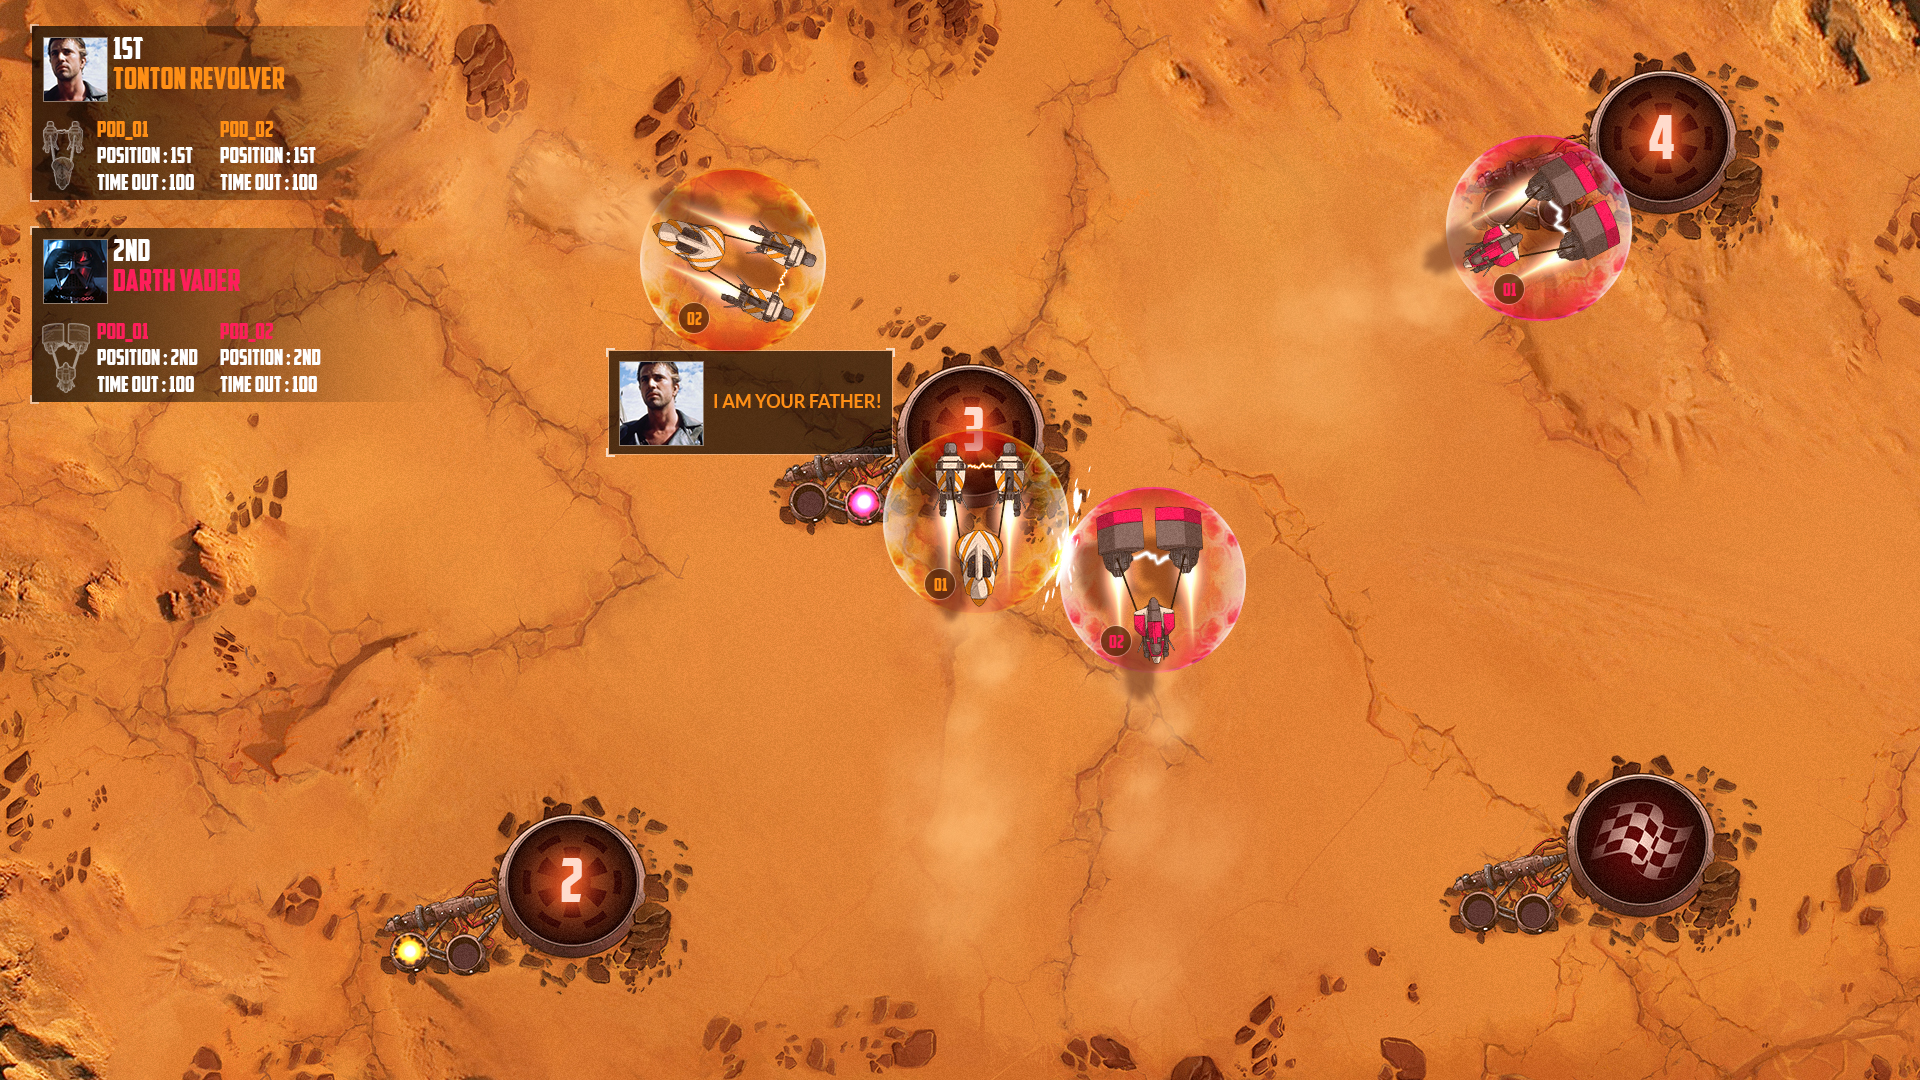
\includegraphics[scale=0.15]{csb-intro.jpg}
\caption{The Universe of Coders Strike Back}
\label{threadsVsSync}
\end{figure}


\subfile{maps}
\subfile{podmove}
\subfile{heaviside}


\bibliographystyle{plain}
\bibliography{references}
\end{document}